\chapter{Forecasting for Decisions}

\begin{weekbox}
\textbf{Theme.} Forecast the quantity the decision needs, over the horizon it needs, and measure the errors honestly,
because next week those errors become safety stock.\\
\textbf{Outcomes.} LO4.\quad \textbf{Tools.} statsforecast, LightGBM, pandas.\\
\textbf{Data.} Mboa daily sales (72 series, known structure); Online Retail II weekly demand of 157 A-class items (real).\\
\textbf{Lab.} Rolling-origin evaluation of baselines, exponential smoothing, intermittent-demand methods and a LightGBM
benchmark; calibrated prediction intervals; export of forecast errors for Week 4.\\
\textbf{Deliverable.} Lab notebook; \textbf{capstone checkpoint 1} (proposal approved, data audit, baseline).
\end{weekbox}

\begin{timetable}
0:00--0:20 & Briefing & ``Our forecast is 85\% accurate.'' Accurate at what, over what horizon, for which decision?\\
0:20--1:10 & Concepts & Horizon and level, rolling-origin validation, error metrics, ETS, Croston, global ML, intervals\\
1:10--2:40 & Guided lab & Lab 3, Steps 1--5 (break at 1:55)\\
2:40--3:40 & Challenge & Exercises 3.3--3.7; capstone checkpoint 1 conversations\\
3:40--4:00 & Debrief & Which model would you deploy for the 157 items, and why not the most complex one?\\
\end{timetable}

\section{What to forecast}
A forecast is an input to a decision, so the decision fixes four choices before any model is fitted.

\begin{enumerate}[nosep]
\item \textbf{Quantity.} Demand, not sales (Week 1). For a perishable product, the whole distribution, because the
order quantity is a quantile of it (Week 4).
\item \textbf{Horizon.} The time between deciding and the end of what the decision covers. For replenishment it is the
\emph{protection interval}: lead time plus review period. A 1-day-ahead forecast is useless for an order that
arrives in 7 days.
\item \textbf{Level.} SKU--store--day for shelves; SKU--warehouse--week for purchasing; category--month for budgets.
Errors shrink as you aggregate, which is why a planner should forecast at the level the decision is made.
\item \textbf{Cost of error.} Symmetric loss (MAE) suits staffing with equal over- and under-costs; asymmetric costs
call for a quantile and the pinball loss.
\end{enumerate}

\section{Honest validation}
\subsection{Rolling-origin evaluation}
A forecast is tested exactly as it will be used: fit on data up to a cutoff, forecast the next $h$ periods, move the
cutoff forward, repeat. Random $k$-fold cross-validation leaks the future into the past and must not be used on time
series.

\begin{figure}[H]
\centering
\begin{tikzpicture}[x=0.37cm,y=0.5cm]
  \foreach \r/\c in {0/20,1/23,2/26,3/29}{
    \fill[navy!80] (0,-\r) rectangle (\c,-\r+0.7);
    \fill[orange] (\c,-\r) rectangle (\c+3,-\r+0.7);
    \fill[slate!25] (\c+3,-\r) rectangle (32,-\r+0.7);
    \node[font=\sffamily\scriptsize,anchor=east] at (-0.3,-\r+0.35) {window \the\numexpr\r+1\relax};}
  \node[font=\sffamily\scriptsize,text=white] at (10,0.35) {training data up to the cutoff};
  \node[font=\sffamily\scriptsize,text=orange,anchor=west] at (32.3,-1.15) {$h$ periods forecast};
  \draw[-{Latex},slate] (0,-3.9) -- (32.5,-3.9) node[right,font=\sffamily\scriptsize]{time};
\end{tikzpicture}
\caption{Rolling-origin evaluation with four windows and step $h$. Each window is one honest test.}
\end{figure}

\begin{pitfall}{Leakage in features}
A feature is legal only if it is known when the forecast is made. For an $h$-week-ahead forecast, last week's demand
is \emph{not} known for weeks $2,\dots,h$. Build every lag and rolling mean from data at least $h$ periods old, or
forecast recursively. Promotions are legal only if they are planned before the cutoff.
\end{pitfall}

\subsection{Error metrics}
\begin{keyformula}{Forecast error metrics ($e_t=\hat y_t-y_t$)}
\begin{tabular}{@{}L{3.6cm}L{5.2cm}L{4.6cm}@{}}
WAPE & $\sum|e_t|\,/\sum y_t$ & scale-free, robust to zeros; our headline metric\\
Bias & $\sum e_t\,/\sum y_t$ & sign tells under- or over-forecasting\\
MASE & $\mathrm{MAE}/\mathrm{MAE}_{\text{naive, in-sample}}$ & $<1$ beats the naive method\\
RMSE & $\sqrt{\tfrac1n\sum e_t^2}$ & penalises large errors; same units as $y$\\
Pinball loss at $\tau$ & $\tfrac1n\sum \max\{\tau(y_t-q_t),(1-\tau)(q_t-y_t)\}$ & scores a quantile forecast $q_t$\\
\end{tabular}
\smallskip
Avoid MAPE on intermittent demand: one week with $y_t=0$ makes it infinite.
\end{keyformula}

Accuracy and bias are different failures. A forecast with 30\% WAPE and zero bias produces stock-outs and overstocks
that roughly cancel; a forecast with 20\% WAPE and $-10\%$ bias produces stock-outs every week. Always report both.

\section{Methods}
\subsection{Baselines you must beat}
\emph{Naive} ($\hat y_{t+h}=y_t$), \emph{seasonal naive} ($\hat y_{t+h}=y_{t+h-m}$), \emph{window average} (mean of the last
$k$ periods). They take one line of code and are surprisingly hard to beat on noisy data. A model that cannot beat
them by a margin worth its maintenance should not be deployed.

\subsection{Exponential smoothing (ETS)}
Simple exponential smoothing updates a level, $\ell_t=\alpha y_t+(1-\alpha)\ell_{t-1}$, and forecasts it flat. Holt adds
a trend and Holt--Winters a seasonal component. The ETS framework writes each variant as a state-space model with
additive or multiplicative error, trend and season; \texttt{AutoETS} chooses among them by AICc. Because ETS is a
statistical model it also gives prediction intervals.

\subsection{Intermittent demand}
When many periods are zero, a smoothed average spreads demand thinly over every period. \textbf{Croston's method}
smooths separately the size of non-zero demands $z$ and the interval between them $p$ and forecasts the rate $z/p$.
\textbf{ADIDA} aggregates the series into non-overlapping buckets until zeros disappear, forecasts the aggregate,
and disaggregates. Both target the \emph{average} rate, which is what a reorder decision needs.

\subsection{Global machine-learning models}
One LightGBM model trained on all series at once, with lags, rolling means and calendar features, learns patterns
shared across items. Global models won the M5 competition on Walmart data (2020), but only with careful feature
engineering and many related series. You know how to fit them; in this course their role is to be honest
benchmarks. Use the Tweedie or Poisson objective for counts with zeros.

\subsection{Prediction intervals and quantiles}
A decision under uncertainty needs a distribution, not a point. Three ways to get one:
\begin{itemize}[nosep]
\item model-based intervals (ETS, ARIMA): $\hat y\pm z_{1-\alpha/2}\hat\sigma_h$, valid if the model is right;
\item \textbf{conformal intervals}: take the empirical quantiles of past out-of-sample errors at the same horizon
and add them to the point forecast; assumption-light and model-agnostic;
\item quantile models: fit the $\tau$-quantile directly with the pinball loss (LightGBM's quantile objective).
\end{itemize}
Always check \emph{coverage}: an 80\% interval should contain about 80\% of new observations. Undercoverage means your
safety stock will be too small.

\begin{realcase}{Weather, hurricanes and Pop-Tarts}
In 2004 the \emph{New York Times} reported that Walmart, mining past sales before hurricanes, found that sales of
strawberry Pop-Tarts rose about sevenfold ahead of a storm, alongside beer, and stocked trucks accordingly. The lesson
is not the snack: exogenous drivers (weather, holidays, school calendars, paydays) often matter more than the choice of
model. Open-Meteo provides historical weather for Douala or Yaoundé free and without a key
(\url{https://archive-api.open-meteo.com/v1/archive?latitude=4.05&longitude=9.70&...}).
\end{realcase}

% ------------------------------------------------------------------ LAB
\section{Practical Lab 3: Forecasting 72 known and 157 real series}
\begin{labbox}{Practical lab --- rolling-origin forecasting with statsforecast}
\textbf{Goal.} Part A checks the workflow on Mboa, where the demand structure is known. Part B forecasts real, lumpy
demand and keeps the errors for Week 4. \textbf{Files.} \texttt{data/sales.csv},
\texttt{real/weekly\_demand\_AXY.parquet} (from Lab 1). \textbf{Time.} 90 minutes; Step 2 runs for about
1--2 minutes on Colab.
\end{labbox}

\subsection*{Part A --- Mboa: does the workflow find what we planted?}
\step{Step 1: Package the Week 1 cleaning as a function}
\codeout{lab3_s1}{A reusable cleaning function and the long-format panel.}

\step{Step 2: Baselines versus ETS, 14 days ahead}
\codeout{lab3_s2}{Six rolling 14-day windows at the end of 2024 for all 72 store--product series.}
\interp{AutoETS with weekly seasonality cuts WAPE from 36\% (naive) to 27\%; MASE below 1 means it beats the
seasonal-naive benchmark. Every method under-forecasts (negative bias), because the test windows cover
October--December and the generator plants an 18\% December uplift that two years of daily data and a weekly model
cannot learn. A planner would add a December adjustment or a yearly regressor. Knowing the truth lets us see
\emph{why} the model is wrong.}

\subsection*{Part B --- Real lumpy demand}
\step{Step 3: Methods for intermittent demand, 4 weeks ahead}
\codeout{lab3_s3}{Eight rolling 4-week windows, April--November 2011, 157 items.}
\interp{Real demand is hard: the best WAPE is 53\%. Croston and ADIDA win narrowly over an 8-week moving average and
SES, with almost no bias. Seasonal naive is worst (+32\% bias): copying last year's week fails for a catalogue that
changes every season. MASE of 0.70 says the good methods cut the naive error by 30\%.}

\step{Step 4: A LightGBM benchmark}
\codeout{lab3_s4}{One global model, retrained at each cutoff, using only features at least four weeks old.}
\interp{LightGBM matches the simple methods on WAPE but has a $-7.8\%$ bias: it under-forecasts the autumn ramp-up.
With 157 short series, the global model has little to learn from. This is the common outcome on small real problems,
and the reason the course insists on baselines.}

\begin{pitfall}{Declaring victory on a 0.5-point difference}
53.15\% versus 53.78\% is noise. Before choosing a model on accuracy, check the spread of errors across windows (or a
Diebold--Mariano test), then prefer the simpler, cheaper, more explainable method.
\end{pitfall}

\step{Step 5: Calibrated intervals and the hand-off to Week 4}
\codeout{lab3_s5}{Conformal intervals, an honest coverage check, and saving the errors.}
\begin{figure}[H]\centering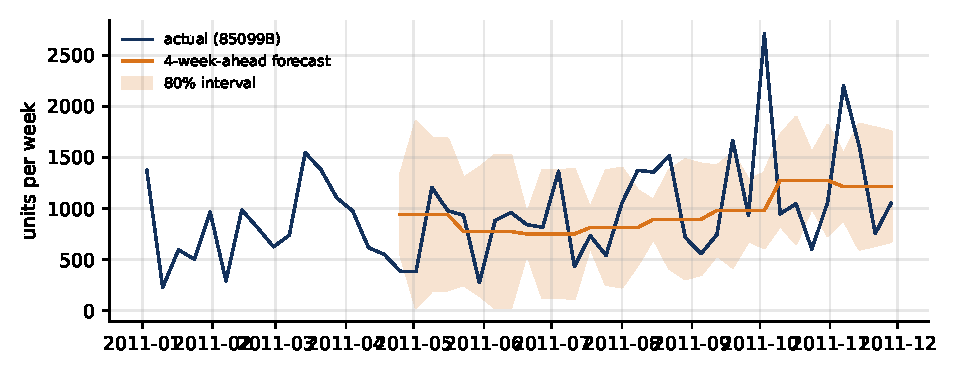
\includegraphics[width=0.92\linewidth]{../figs/lab3_sku.pdf}
\caption{The highest-volume item: actual weekly demand, 4-week-ahead forecasts and 80\% conformal intervals.}\end{figure}
\interp{The intervals cover 74.5\% instead of 80\%, and 85.5\% instead of 95\%. They were calibrated on calmer weeks and
then met the autumn peak. Undercoverage of this size means a safety stock set from these errors will deliver less
service than promised, which is exactly what Lab 4 will show.}

\paragraph{So what (model answer)} \emph{For the 157 key items, a simple intermittent-demand method (ADIDA) forecasts
four weeks ahead with 53\% WAPE and no bias, as well as a machine-learning model and with less effort. Errors are
large and grow in the autumn peak, so stock decisions must be built on the error distribution, not on the point
forecast, and the error estimate must be refreshed before the peak.}

% ------------------------------------------------------------------ EXERCISES
\section{Exercises}
\begin{enumerate}[label=\textbf{3.\arabic*},leftmargin=2.4em]
\item \emph{(Concept)} A supplier delivers 10 days after an order and Mboa orders every Monday. What forecast horizon
matters for the order? Why is the accuracy of tomorrow's forecast irrelevant?
\item \emph{(Metrics)} For actuals $(0,4,0,6)$ and forecasts $(2,2,2,2)$, compute MAE, WAPE, bias and MAPE. Which metric
breaks, and why?
\item \emph{(Pinball)} Show that the constant $q$ minimising the average pinball loss at $\tau$ over a sample is the
$\tau$-quantile of the sample.
\item \emph{(Mboa)} Add a December dummy as an exogenous regressor (\texttt{AutoARIMA} accepts exogenous columns) for
rice in all stores. How much does the bias in Step 2 change?
\item \emph{(Real data)} Repeat Step 3 for B-class items. Does the ranking of methods change?
\item \emph{(Quantiles)} Fit a LightGBM quantile model at $\tau=0.9$ in Step 4 and measure its coverage. Compare with
the conformal 80\% upper bound.
\item \emph{(Exogenous data)} Download daily Douala temperature and precipitation for 2023--2024 from Open-Meteo and test
whether rain improves the water (P05) forecast at Douala Akwa. Remember the result is synthetic: what would you
expect, and what did you find?
\end{enumerate}

\section{Take-home assignment 3 and capstone checkpoint 1}
\begin{enumerate}[nosep]
\item For the 157 items, produce a one-page forecast report for the purchasing manager: recommended method, accuracy
and bias by ABC--XYZ class, and the items you would \emph{not} trust the forecast for.
\item \textbf{Checkpoint 1} (in class): approved decision statement, data audit table (rules and counts), and a baseline
result: the number your capstone must beat.
\end{enumerate}
